\documentclass[11pt]{article}
%%%%%%%%%%%%%%%%%%%%%%%%%%%%%%%% Algunos Paquetes Necesarios 
\usepackage{fancyhdr, graphicx, wrapfig,lipsum}
\usepackage[utf8]{inputenc} % Tildes
\usepackage[spanish]{babel} % Language
\usepackage{babelbib} % Bibliografia español
\usepackage[margin=1in]{geometry} % Margins														
\usepackage{amssymb}
\usepackage{amsmath, amsthm, amsfonts}
\usepackage[table]{xcolor} % Color table
\usepackage{longtable} % Table accross multiple pages
\usepackage{hyperref}  % Use Hyperlinks
\usepackage{enumerate} % Reduce space in enumerate
\usepackage{txfonts}
\setlength{\parindent}{0in}
\decimalpoint

\usepackage{cancel}
\usepackage{float}

%%%%%%%%%%%%%%%%%%%%%%%%%%%%%%%%%%%%%%%%%%%%%%%%%%%%%%%%%%%%%%%%%%%%%%%%%%%%%%%%%%%%%%%%%%%%%%%%%%%%%%%%%%%%%%%%%%%%%%%%%%%%%%%%%%%%%%%%%%%%%%%%%%%%%%%%%%%%%%%%

%%%%%%%%%%%%%%%%%%%%%%%%%%%%%%%%%%%%%%%%%%%%%%%%%%%%%%%%%%%%%%%%%%%%%%%%%%%%%%%%%%%%%%%%%%%%%%%%%%%%%%%%%%%%%%%%%%%%%%%%%%%%%%%%%%%%%%%%%%%%%%%%%%%%%%%%%%%%%%%%
\newcommand{\myName}{}
\newcommand{\myDate}{}
\newcommand{\myCourse}{}


%\newcommand{\R}{\mathbb{R}}
%\newcommand{\F}{\mathbf{F}}
%\newcommand{\vi}{\mathbf{\hat{i}}}
%\newcommand{\vj}{\mathbf{\hat{j}}}
%\newcommand{\vk}{\mathbf{\hat{k}}}
%\newcommand{\op}{\sigma\sqrt{2\pi}}
%%%%%%%%%%%%%%%%%%%%%%%%%%%%%%%%%%%%%%%%%%%%%%%%%%%%%%%%%%%%%%%%%%%%%%%%%%%%%%%%%%%%%%%%%%%%%%%%%%%%%%%%%%%%%%%%%%%%%%%%%%%%%%%%%%%%%%%%%%%%%%%%%%%%%%%%%%%%%%%%

%%%%%%%%%%%%%%%%%%%%%%%%%%%%%%%%%%%%%%%%%%%%%%%%%%%%%%%%%%%%%%%%%%%%%%%%%%%%%%%%%%%%%%%%%%%%%%%%%%%%%%%%%%%%%%%%%%%%%%%%%%%%%%%%%%%%%%%%%%%%%%%%%%%%%%%%%%%%%%%%
%%%%%%%%%%%%%%%%%%%%%%%%%%%%%%%%%%% Tema - BEGIN
\newtheoremstyle{Tema}% name of the style to be used
  {5mm}% measure of space to leave above the theorem. E.g.: 3pt
  {10mm}% measure of space to leave below the theorem. E.g.: 3pt
  {}% name of font to use in the body of the theorem
  {}% measure of space to indent
  {\bfseries}% name of head font
  {\newline}% punctuation between head and body
  {30mm}% space after theorem head
  {}% Manually specify head

\theoremstyle{Tema} \newtheorem{Tema}{Tema} %%%%% Template para Temas
\theoremstyle{Tema} \newtheorem{Serie}{Serie}              %%%%%  Template para Series de ejercicios
\theoremstyle{Tema} \newtheorem{Ejercicio}{Ejercicio}    %%%%%  Template para Ejercicios
%%%%%%%%%%%%%%%%%%%%%%%%%%%%%%%%%%% Tema - END


%%%%%%%%%%%%%%%%%%%%%%%%%%%%%%%%%%% Encabezado - BEGIN %%%%%%%%%%
\fancypagestyle{firststyle}
{
\renewcommand{\headrulewidth}{1.5pt}
\fancyhead[R]{
			\textbf{Universidad de San Carlos de Guatemala} \\
			\textbf{Escuela de Ciencias Físicas y Matemáticas}\\
			\textbf{\myCourse }  \\  %%%%%%%%%% Agregar nombre del curso 
			\textbf{\myDate}   %%%%%%%%%%%%%%%%%%%%%% Agregar fecha en formato: Enero 15, 2015
			}
\fancyhead[L]{ 
	\includegraphics[height=1.6 cm]{/home/jorgealejandro/Templates/ECFM.png} \\
	\textbf{Jorge Alejandro Rodriguez Aldana}\\
	\textbf{201804766} 
	}
}
%%%%%%%%%%%%%%%%%%%%%%%%%%%%%%%%%%% Encabezado - END %%%%%%%%%%

%%%%%%%%%%%%%%%%%%%%%%%%%%%%%%%%%%% Encabezado (pagina 2 en adelante) - BEGIN %%%
\fancypagestyle{allStyle}
{
\renewcommand{\headrulewidth}{1pt}
\fancyhead[R]{
			\emph{\myName $-$ \myCourse} %%%% Modificar número de examen parcial y nombre del curso
			}
\fancyhead[L]{}  
\fancyfoot[C]{}
\fancyfoot[R]{\thepage}
}
%%%%%%%%%%%%%%%%%%%%%%%%%%%%%%%%%%% Encabezado (pagina 2 en adelante) - END %%%

\date{}
\setlength{\headheight}{0.8in} % fixes \headheight warning

%%%%%%%%%%%%%%%%%%%%%%%% BEGIN %%%%%%%%%%%%%%
\begin{document}

\pagestyle{allStyle}

\thispagestyle{firststyle}
%%%%%%%%%%%%%%%%%%%%%%%%%%%%%%%%% Titulo - BEGIN
\begin{center}
\LARGE
\textsc{\myName} % Modificar el Número del examen parcial
\medskip
\hrule height 1.5pt
\end{center}
%%%%%%%%%%%%%%%%%%%%%%%%%%%%%%%%%%%%%%%%%%%%%%%%%%%%%%%%%%%%%%%%%%%%%%%%%%%%%%%%%%%%%%%%%%%%%%%%%%%%%%%%%%%%%%%%%%%%%%%%%%%%%%%%%%%%%%%%%%%%%%%%%%%%%%%%%%%%%%%%


%%%%%%%%%%%%%%%%%%%%%%%%%%%%%%%%% Instrucciones - BEGIN
\vspace{0.1 in}

\begin{abstract}
    NO SE NOS OLVIDE HACER EL RESUMEN
\end{abstract}

\maketitle

\section{Introducción}

Un aparente problema, surge cuando tenemos dos partículas entrelazadas, las alejamos, y medimos una de ellas, colapsando el estado de ambas. 
Aparentemente, la información ha viajado de forma instantánea, violando las leyes de la relatividad especial. 

Hacer un análisis matemático al respecto es importante, y así dar una justificación al por que se busca la aprobación de una teoría: la mecánica cuántica no es local.

Esta no es más una teoría, ya que ha sido demostrada en disversas situaciones. Pero demostrar que los eventos no tienen una relación causal, es un buen ejercicio que nos da la dirección a la inminente conclusión que la mecánica cuántica es una teoría no local, y por tanto, no contradice a la relatividiad especial.


\section{Paradoja de EPR}

% Partamos, suponiendo que la mecánica cuántica es una teoría local, de modo que 

Si tenemos dos partículas entrelazadas, sabemos que al medir una de ellas, se definirá en un estado, y por tanto, la otra también lo hará. El problema con esto, es que, aparentemente, tenemos dos eventos directamente relacionados, ocurriendo al mismo tiempo, lo que parece una contradicción a la Relatividad.

% Veamos cual es el error de este planteamiento; para que la mecánica cuántica siga las reglas de la Relatividad, debe ser una teoría local, y por tanto

% \input{Geogebra/EPR-Bell.tex}

\begin{figure}[H]
    \centering
    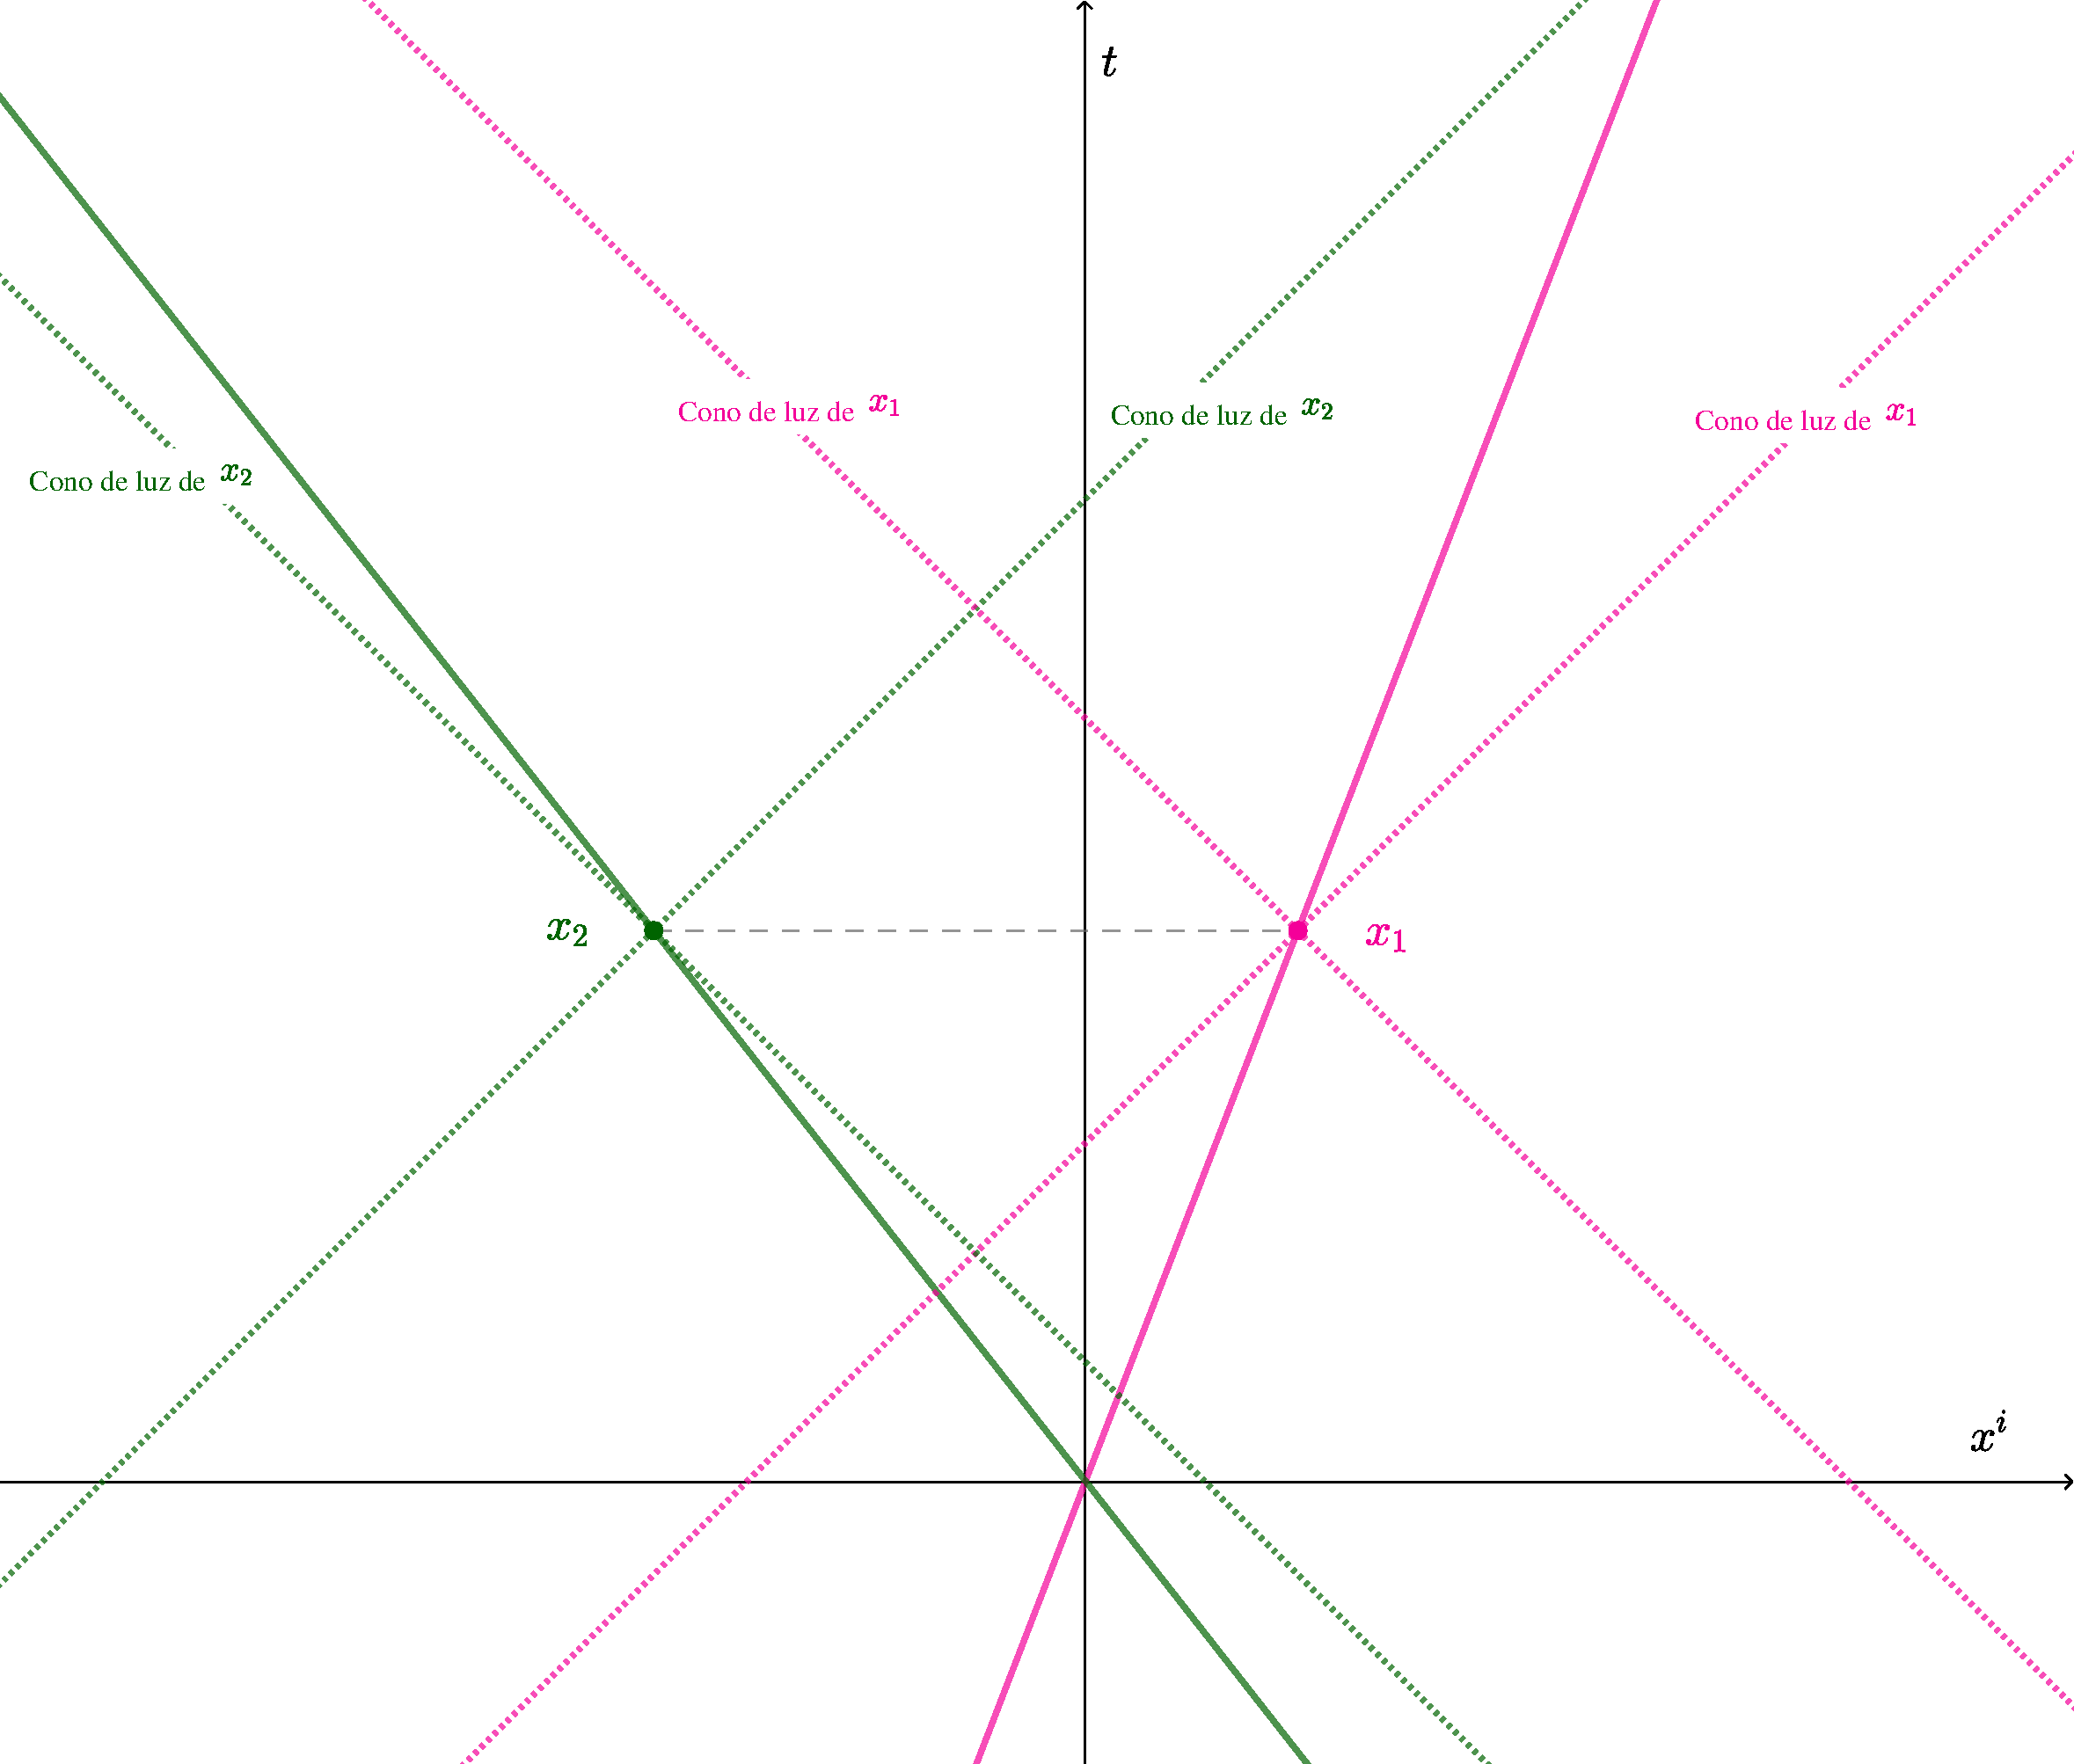
\includegraphics[width=0.4\textwidth]{Graphics/SpaceLike.pdf}
    \label{fig:SpaceLike}
    \caption{Diagrama de Minkowski}
\end{figure}
\bigskip

Veamos este planteamiento con más rigurosidad matemática:

\medskip

Sean $\mathbf{x_1}$ y $\mathbf{x_2}$, dos partículas observadas por un mismo observador en un sistema inercial, que se entrelazan en $t=0$ y luego se alejan a velocidades $\mathbf{v_1}$ y $\mathbf{v_2}$ respectivamente. Entonces tenemos:

\begin{align*}
    \mathbf{x_1} &= \left(x^0_1,x^1_1,x^2_1,x^3_1\right)\\
    \mathbf{x_2} &= \left(x^0_2,x^1_2,x^2_2,x^3_2\right)
\end{align*}

Pero, al ser observados por un mismo observador, partiendo de un mismo evento, entonces: $x^0_1=x^0_2=t$:

\begin{align*}
    \mathbf{x_1} &= \left(t,x^1_1,x^2_1,x^3_1\right)\\
    \mathbf{x_2} &= \left(t,x^1_2,x^2_2,x^3_2\right)
\end{align*}

Y suponiendo una velocidad constante, entonces $x^i_n=tv^i_n$:

\begin{align}
    \mathbf{x_1} &= \left(t,tv^1_1,tv^2_1,tv^3_1\right)\\
    \mathbf{x_2} &= \left(t,tv^1_2,tv^2_2,tv^3_2\right)
\end{align}

Calculemos entonces $\Delta x^\alpha$

\begin{align*}
    \Delta x^\alpha 
        &:= \left(x^\alpha_2-x^\alpha_1\right)\\
    \Delta x^0
        &= \left(t-t\right)=0\\
    \Delta x^i
        &= \left(x^i_2-x^i_1\right)\\
        &= \left(tv^i_2-tv^i_1\right)\\
        &= t\left(v^i_2-v^i_1\right)\\
        &= t\Delta v^i
\end{align*}

Calculemos ahora $\Delta s^2$

\begin{align*}
    \Delta s^2 
        &:= -\eta_{\alpha\beta}\Delta x^\alpha \Delta x^\beta\\
        &=-\eta_{00}~\cancelto{0}{\left(\Delta x^0\right)^2}-\cancelto{\delta_{ij}}{\eta_{ij}}~~~~~\left(\Delta x^i\Delta x^j\right)\\
        &=0-\delta_{ij}\left(\Delta x^i\Delta x^j \right)\\
        &=\sum_{i=1}^3-\left(\Delta x^i\right)^2\\
        &=-t^2\sum_{i=1}^3 \left(\Delta v^i\right)^2\\
        &=-t^2\left[\left(\Delta v^1\right)^2+\left(\Delta v^2\right)^2+\left(\Delta v^3\right)^2\right]\\
        &\leq0
\end{align*}

El caso de la igualdad solo se da en $t=0$ o si las velocidades de ambas partículas son las mismas, de modo que $\Delta v^i = 0~~\forall~i\in[1,3]$

Y por tanto, en el caso que las velocidades sean distintas, la métrica de Minkowski es menor a cero, es decir, los eventos $x_1$ y $x_2$ no tienen una relación causal. Y al estar correlacionados, esto es una aparente violación de la teoría de la Relatividad.



\end{document} %%%%%%%%%%%%%%%%%%%%%%%% BEGIN%%%%%%%%%%%%%%